\documentclass[11 pt, a4paper]{article}

\usepackage[left=1.5cm,top= 1.5cm,right= 1.5cm,bottom=1.5cm]{geometry}
\usepackage[spanish]{babel}
\usepackage{amsthm}
\usepackage{graphicx}
\theoremstyle{definition}
\newtheorem{definicion}{Definici\'on}[section]
\graphicspath{{img/}}
\usepackage[utf8]{inputenc} 
\usepackage{amsmath,amssymb,amsfonts,latexsym} %Soporte para símbolos y font matemáticos
\usepackage{float}
\usepackage{enumerate}
% \usepackage[options]{algorithm2e}
\DeclareGraphicsExtensions{.pdf,.png,.jpg}
\DeclareGraphicsRule{.wmf}{bmp}{}{}

\author{Trinidad Hern\'andez Norma Ver\'onica \\
        Vargas Mu\~noz Jos\'e de Jes\'us \\
        Vilchis Dom\'inguez Miguel Alonso}
\title{Tarea 1}
\begin{document}
\maketitle

\section{Ejercicios}

\begin{enumerate}

    \item \textbf{Explicar la complejidad de los problemas tipo NP, NP-Completos y NP-Duros para panaderos.}\\
            \textbf{Reducciones} \\ 
            A un panadero se le encomienda la tarea de cocinar galletas con forma de cuadrado, pero sabe que si
            le da dicha forma a las galletas, estas no se cocinar\'an del centro. Por el contrario, sabe que si cocina
            galletas de forma circular estas se cocinar\'an de una manera uniforme. ?`C\'omo entrega el panadero galletas
            cuadradas y cocidas del centro? Haciendo uso de una reducci\'on. \par

            \definicion{ Sean $P$ y $Q$ dos problemas. Sup\'ongase que un ejemplar arbitrario $E$ de $P$ puede solucionarse convirtiendo al ejemplar $E$ en un ejemplar $E'$ de $Q$, resolviendo para $E'$ y reduciendo la soluci\'on $S'$ en la soluci\'on $S$ para $E$. Si existen algoritmos $C_{Ej}$, para convertir un ejemplar $E$ en otro $E'$, y $C_{Sol}$ para convertir la soluci\'on $S'$ en $S$, se dice entonces que existe una reducci\'on de $P$ en $Q$, la cual se denota como $P \propto Q$.} \par

            El panadero toma la masa de galletas $(E)$ y utiliza un cortador $(C_{Ej})$ para darles forma circular
            $(E')$. Cocina esta masa con formas redondas en el horno y obtiene galletas perfectas $(S)$. Cuando las galletas se enfr\'ian, el panadero utiliza un cuchillo para cortarlas $(C_{Sol})$ y obtener ejemplares cuadrados $(S')$. Nuestro panadero acaba de aplicar el \emph{Algoritmo de Reducci\'on (o de Simplificaci\'on)} para resolver su problema. Tal algoritmo es usado cuando $P$ es muy dif\'icil de resolver de manera directa y
            $Q$ es m\'as f\'acil.

            \begin{figure}[h]
                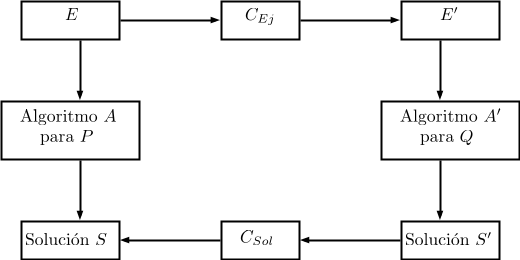
\includegraphics[width=80mm]{Reduc_P_en_Q.png}
                \centering
                \caption{Reducci\'on de $P$ en $Q$: $P \propto Q$}
                \label{fig:PQ_Red}
            \end{figure}


            \begin{figure}[h]
                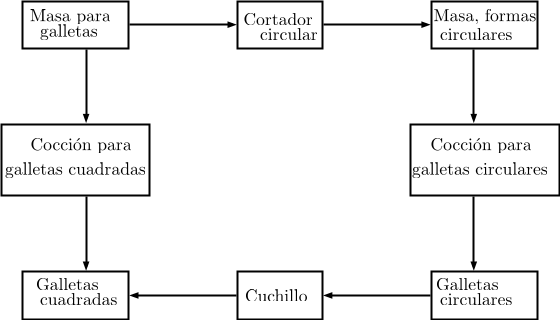
\includegraphics[width=80mm]{Reduc_P_en_Q_Pan.png}
                \centering
                \caption{Reducci\'on de $P$ en $Q$ para panaderos}
                \label{fig:PQ_Red_Pan}
            \end{figure}

            Supongamos que el panadero tarda 2 segundos en cortar una porción de masa en forma de una galleta circular,
            y supongamos que le toma 4 segundos cortar con cuchillo una galleta circular para obtener una cuadrada.
            Cortar $n$ galletas circulares le tomar\'a al panadero $T(n) = 2n$ segundos, y cortarlas despu\'es en galletas
            cuadradas le tomar\'a $T(n) = 4n$ segundos. Se dice que ambas transformaciones son \emph{polinomiales}, ya
            que el tiempo que toma convertir el ejemplar de un problema a otro ($T(n) = 2n$), as\'i como convertir la soluci\'on de un problema en la soluci\'on de otro ($T(n) = 4n$), es polinomial. Por desempe\~no computacional de orden polinomial nos referimos a que es posible expresar el tiempo de transformaci\'on como un polinomio que est\'a en funci\'on del tama\~no de la entrada. En este caso, del n\'umero de galletas. \par

            Nuestro panadero puede no saber c\'omo cocinar galletas cuadradas en un horno, pero s\'i c\'omo cocinarlas
            circulares y despu\'es cortarlas. El panadero le ocultar\'a a los dem\'as que desconoce la manera de cocinar galletas cuadradas en el horno y esto no le angustia: el panadero puede obtener galletas cuadradas de otra forma, en tiempo polinomial, y eso es lo importante. Nuestra idea se resume en el siguiente teorema.\\
            \textbf{Teorema.} Si $L_1$ es polinomialmente reducible a $L_2$ y existe un algoritmo polinomial para $L_2$, entonces existe un algoritmo polinomial para $L_1$. $\square$ \\

            \textbf{El No Determinismo} \\
            Nuestro panadero estricto sigue recetas al pie de la letra para sus galletas, lo cual le garantiza exactamente las mismas galletas cada vez, siempre y cuando use los mismos ingredientes. Este panadero sigue algorimos deterministas cada vez que cocina. En t\'erminos de computaci\'on, decimos que un algoritmo es \emph{determinista} si para una entrada particular, siempre produce la misma salida, con la m\'aquina subyacente siempre pasando por la misma secuencia de estados. Volviendo a la cocina, el algoritmo determinista del panadero es la receta que sigue, la entrada particular son los ingredientes de sus galletas, la salida es el producto final, la m\'aquina subyacente est\'a representada por sus manos y los utensilios de los que se vale, y la secuencia de estados es la forma que va tomando la masa. \par
            Ahora bien, supongamos que a nuestro panadero se le encarga crear una galleta que sea crujiente en su exterior y suave en su interior. El panadero sabe que este requerimiento particular para la galleta depende de la manera de batir la masa, pero no sabe en espec\'ifico que m\'etodo al aplicarse resultar\'a en la galleta deseada. El panadero modifica la receta como sigue: comienza la preparaci\'on de la galleta como sabe hacerlo y cuando llega el momento de batir tira un dado, el cual le indicar\'a qu\'e t\'ecnica de batido usar. \\

            Un \emph{algoritmo no determinista} tiene todas las operaciones cl\'aiscas de uno determinista, con la adici\'on de una primitiva no determinista llamada \emph{nd-choice}, la cual es usada para manipular selecciones. \\

            Nuestro panadero us\'o una primitiva nd-choice en su receta (algoritmo): el dado. Entonces, dependiendo del resultado del dado se obtiene una galleta distinta. \'El prueba la galleta una vez salida del horno; esto para determinar si result\'o seg\'un los requerimientos. Nuestro panadero acaba de crear, sin saberlo, un algoritmo no determinista de tiempo polinomial. El algoritmo es el siguiente:
            \begin{enumerate}
                \item Aplicar cierto n\'umero de pasos de la receta como suele hacerlo.
                \item Utilizar una primitiva \emph{nd-choice} para hacer un cambio aleatorio a la receta.
                \item Seguir con los pasos de la receta.
                \item \textbf{Verificar} si el producto obtenido es como se deseaba. De ser as\'i, reportar \textbf{s\'i}, y 
                        \textbf{no} en caso contrario.
            \end{enumerate}
            Es importante notar que esta estructura de algoritmo no determinista tiene desempe\~no polinomial porque tanto la aplicaci\'on de la primitiva \emph{nd-choice} como la verificaci\'on toman tiempo polinomial.

            \definicion {La clase de problemas para los cuales existe un algoritmo no determinista cuyo desempe\~no computacional es polinomial (en funci\'on del tama\~no de la entrada) es llamada \textbf{Clase NP}.}

            Supongamos para efectos de nuestro ejemplo que la Clase NP se restringe a la panader\'ia de nuestro personaje.Esto es, la Clase NP se compone de cierto n\'umero de galletas. Digamos que el panadero elige una galleta $X$ y descubre que todas las dem\'as recetas de galletas donde usa su dado (los dem\'as problemas de la clase NP) pueden reducirse a la galleta $X$. Decimos entonces que la galleta es \textbf{NP-Dura.}

            \definicion {Un problema $X$ es llamado \emph{Problema NP-Duro}, \emph{NP-Hard}, si cada problema en NP es polinomialmente reducible en $X$.}

            Ahora supongamos que nuestro panadero conoce una receta de galletas $X$ que es de la clase NP, es decir, utiliza un dado en su preparaci\'on. Supongamos adem\'as que la galleta es NP-Dura, es decir, todas las dem\'as recetas galletas de la Clase NP pueden reducirse en tiempo polinomial a la receta de la galleta $X$. Entonces decimos que nuestra galleta es NP-Dura.

            \definicion {Un problema $X$ es llamado \emph{Problema NP-Completo}, \emph{NP-Complete}, si
                \begin{enumerate}
                    \item el problema $X$ pertenece a NP y
                    \item el problema $X$ es NP-Duro
                \end{enumerate}
            }
          
  \item \textbf{2. ¿Para qué valores de $n$ el algoritmo de inserción directa es mejor que mezcla directa? }
    \[ Inserci\acute{o}n \ directa : \ \ \ 8(n^2)\]
    \[ Mezcla\ directa: \ \ \ 64n*log(n) \]
    \begin{itemize}
     \item \textbf{Respuesta en forma analítica:} \\ 
      Para saber que algoritmo es mejor que otro nos basamos en diferentes 
      métricas en las que podemos cuantificar cual es la cantidad
      de recursos que son requeridos para resolver la tarea. Estos 
      recursos principalmente se dividen en dos, el tiempo de ejecución del
      algoritmo y la cantidad de memoria que el algoritmo requiere.\\
      Implícitamente podemos medir el tiempo de ejecución si conocemos 
      cuantas instrucciones ejecutará el algoritmo, debido  a que 
      cada una de nuestras computadoras puede ejecutar un número determinado
      de instrucciones por segundo, es por ello que para conocer el número
      de segundos que tomará un algoritmo en finalizar queda determinado 
      por:
      \[ Tiempo (s) =\frac{\#\ instrucciones}{\#\ instrucciones\ por\ segundo\ que\ la\ computadora\ ejecuta}\ \ \ \left( \frac{instrucciones}{instrucciones/s} \right) \]
      Por esa razón, para saber que algoritmo es mejor que otro 
      basta con fijarse en el número de instrucciones que cada
      uno de ellos requieren, asumiendo que la misma computadora ejecutara 
      los algoritmos.Es importante notar que   el número de instrucciones 
      es una función que depende de los datos de entrada que se le dan al 
      algoritmo. \\
      Por lo ya descrito, para conocer cuándo el algoritmo de 
      inserción directa es mejor que el algoritmo de mezcla directa se 
      hace una análisis sobre la entrada comparando la cantidad de 
      instrucciones que cada uno de estos requiere.\\
      Con el objetivo de discernir para que valores de $n$ el número 
      de instrucciones del algoritmo de inserción directa es menor
      que el algoritmo de mezcla directa, si definimos $I$ como la 
      función que calcula el número de instrucciones por cada algoritmo 
      basta con resolver la siguiente desigualdad:
       \[ I(Inserci\acute{o}n\ directa) \leq I( Mezcla \  directa) \]
      Es decir:
       \[ 8*n^2 \leq 64n*log(n) \]
      $\Longleftrightarrow$
	\[ n \leq 8*log(n) \]
      Trabajando solo con la igualdad encontraremos el valor de $n$ en 
      el que se deja de cumplir la desigualdad estricta. Es decir:
      \[ n - 8*log(n) = 0 \]
      Dicho algoritmo en realidad está en base 2, debido a que el análisis
      de complejidad de merge sort depende de un árbol binario completo
      es por esa razón que la altura queda representada por $log_2(n)$.
      Si graficamos esta igualdad obtenemos:
      \begin{figure}[H]
         \centering
          %trim left bottom right top
          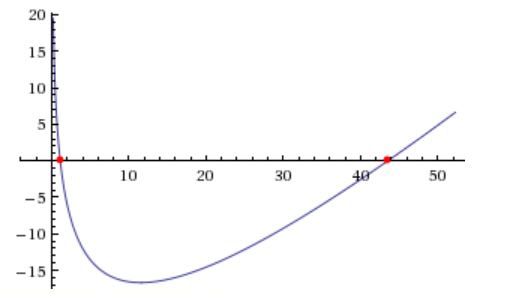
\includegraphics[trim=0cm 0cm 0cm 0cm, width=10cm]{ejercicio2_1.png} 
          \caption{Gráfica $y= n-8*log_2(n)$}
      \end{figure}
      Por lo que, la solución a la igualdad es cuando
      $n =1.0\overline{999}$ y $n=43$, con lo que concluimos que si 
      $2 \leq n \leq 43$, entonces el algoritmo de inserción directa 
      es más mejor que el algoritmo de mezcla.
   

  \item \textbf{Respuesta de manera experimental:} \\ 
Al poner en ejecución el programa se tomo como precaución el
	no trabajar con interfaz gráfica ni con otro programa ejecutandose
	al mismo tiempo para evitar, en medida de lo posible, 
	la intervención de ruido en nuestras mediciones.\\ 
	Realizamos 3 versiones para cada algoritmo, una escrita
	en java, otra escrita en C y una escrita en python. Al 
	hacer la ejecución de nuestro código y graficar el tiempo
	que tardó cada programa, obtenemos los siguientes resultados:
\begin{figure}[H]
         \centering
          %trim left bottom right top
          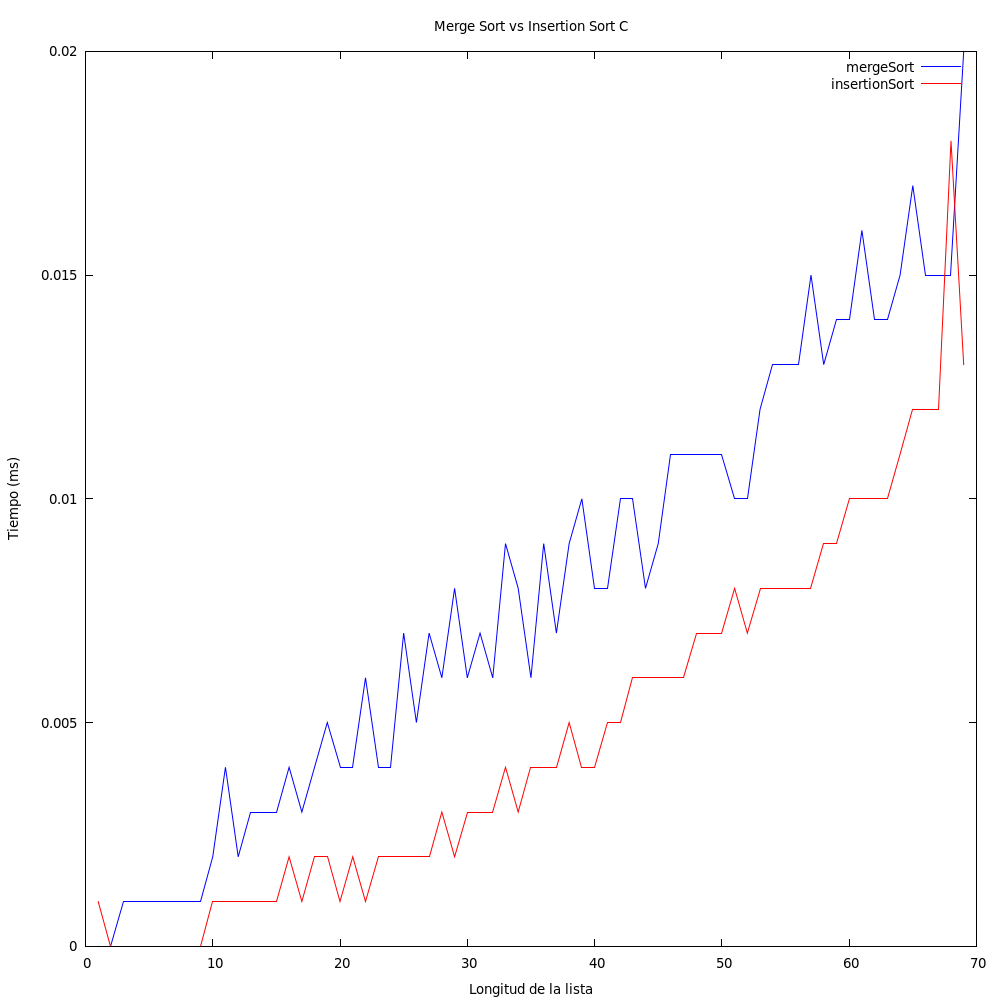
\includegraphics[trim=0cm 0cm 0cm 0cm, width=10cm]{C.png} 
          \caption{Gráfica que muestra tiempo vs longitud de la lista para el lenguaje C}
      \end{figure}
\begin{figure}[H]
         \centering
          %trim left bottom right top
          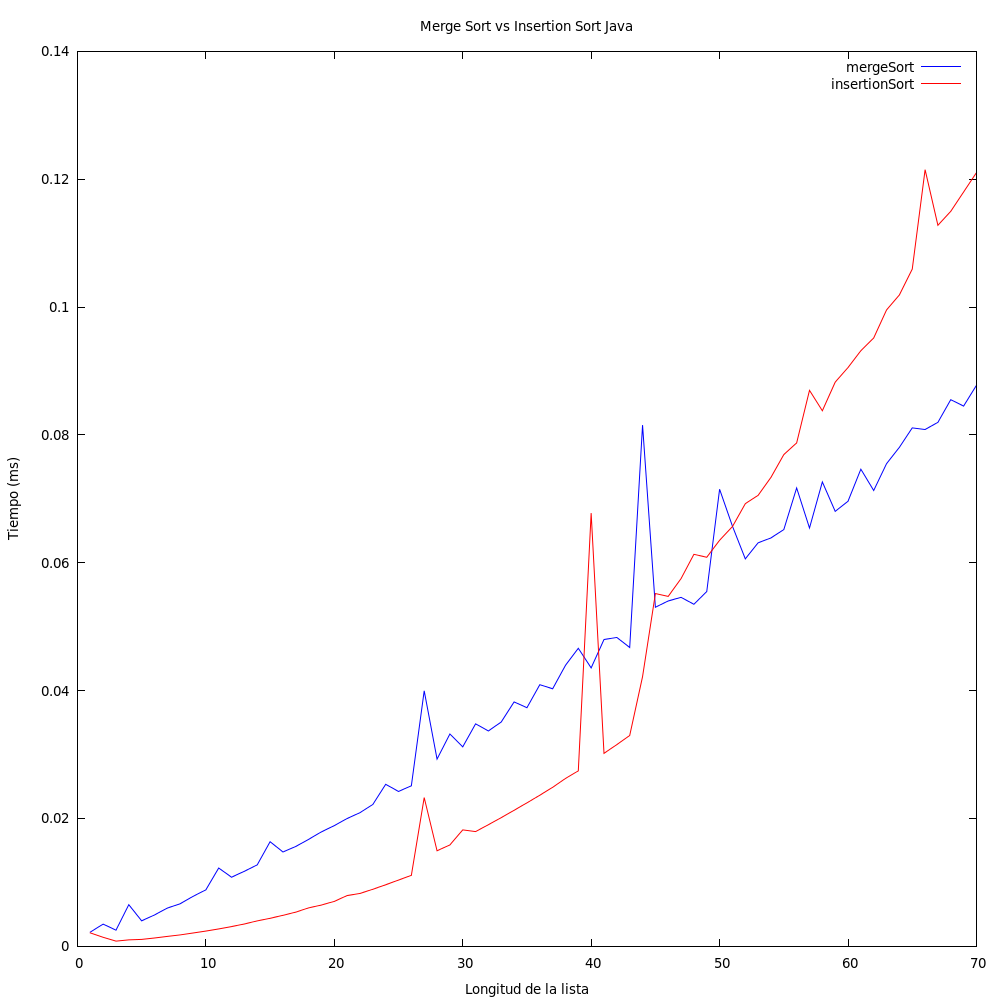
\includegraphics[trim=0cm 0cm 0cm 0cm, width=10cm]{Java.png} 
          \caption{Gráfica que muestra tiempo vs longitud de la lista para el lenguaje Java}
      \end{figure}
\begin{figure}[H]
         \centering
          %trim left bottom right top
          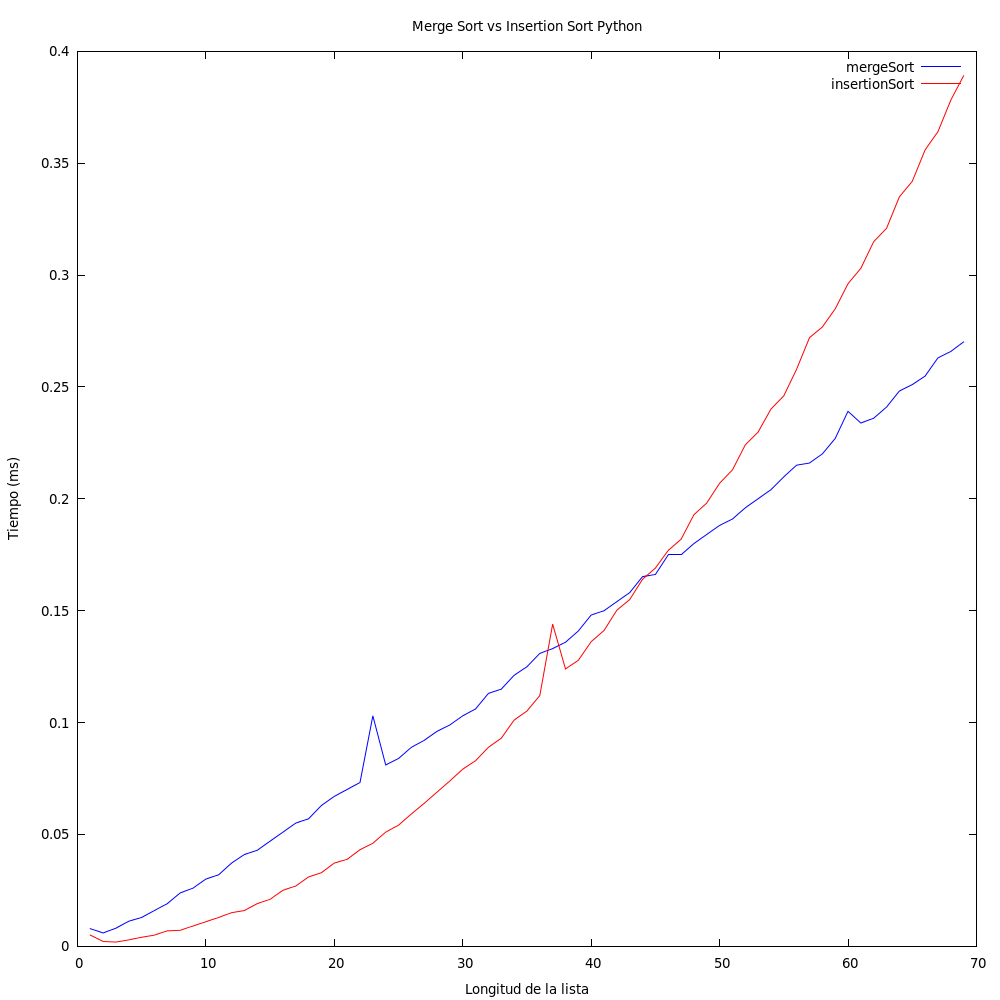
\includegraphics[trim=0cm 0cm 0cm 0cm, width=10cm]{Python.png} 
          \caption{Gráfica que muestra tiempo vs longitud de la lista para el lenguaje Python}
      \end{figure}
	En las gráficas podemos apreciar que para el lenguaje de
	programación Python la cota teórica se respetó totalmente, 
	sin embargo, para C esto no ocurrió, las causas pueden ser
	diversas, pero nos aventuramos a conjeturar que una de las
	posibles razones fue que al generar números aleatorios para
	ordenar, estos pudieron comportarse de tal manera que no
	explotaran el peor caso del algoritmo de Inserción directa,
	dicho caso se presenta cuando los números están acomodados
	de manera inversa al orden natural. 
	
    \end{itemize}
\item \textbf{3. ¿Cuál es el valor más pequeño de $n$, tal que un algoritmo cuyo tiempo de ejecución es $x$ corre más rápido cuyo tiempo de ejecución es $y$?.}\\
Para este ejercicio nos apoyamos en el software Mathematica, la solución se obtuvo mediante el uso de gráficas para las funciones, y encontrando los puntos críticos.\\
    \begin{enumerate}
        \item $x = 100n^2 \\ y = 2^n$ \\
        \begin{figure}[H]
         \centering
          %trim left bottom right top
          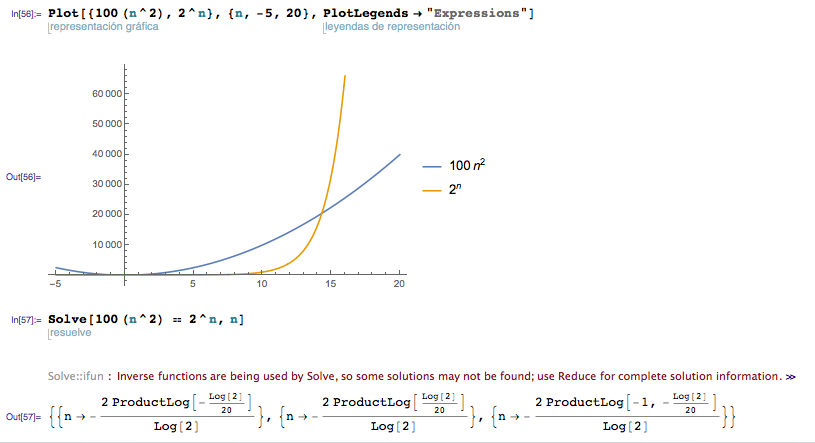
\includegraphics[trim=0cm 0cm 0cm 0cm, width=10cm]{3a.png} 
          \caption{Gráfica y Puntos críticos}
        \end{figure}
        \item $x = 6n^2 \\ y = 32n\log(n)+5n$
        \begin{figure}[H]
         \centering
          %trim left bottom right top
          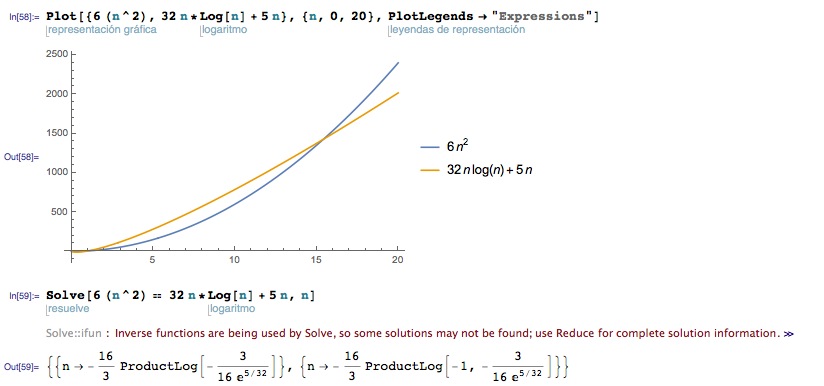
\includegraphics[trim=0cm 0cm 0cm 0cm, width=10cm]{3b.png} 
          \caption{Gráfica y Puntos críticos}
        \end{figure} 
    \end{enumerate}

\item \textbf{4. Ejecutar el algoritmo de Inserción directa y de Mezcla directa para grandes valores de $n$}\\
  Para este ejercicio se tomaron las mismas precauciones que para el ejercicio 2, las iteraciones se realizaron sin
  interfaz gráfica y sin ejecutar otro programa para evitar, hasta donde es posible, el ruido en nuestros datos.\\
  La presentación de los datos la realizamos en forma de gráfica para que los datos sean más fáciles de interpretar. 
   \begin{figure}[H]
         \centering
          %trim left bottom right top
          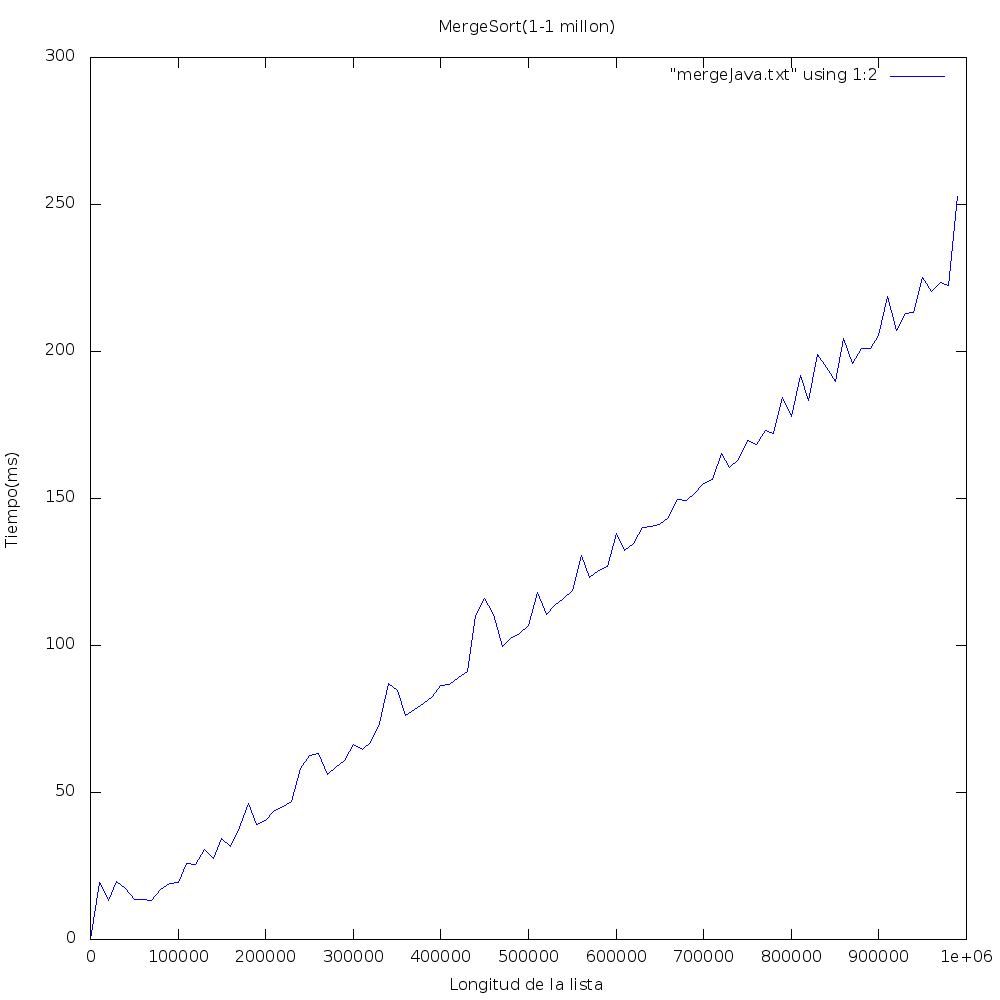
\includegraphics[trim=0cm 0cm 0cm 0cm, width=10cm]{1-1mJava.png} 
          \caption{Gráfica para MergeSort en el lenguaje Java de 1 a 1 millon}
      \end{figure}
      
      
       \begin{figure}[H]
         \centering
          %trim left bottom right top
          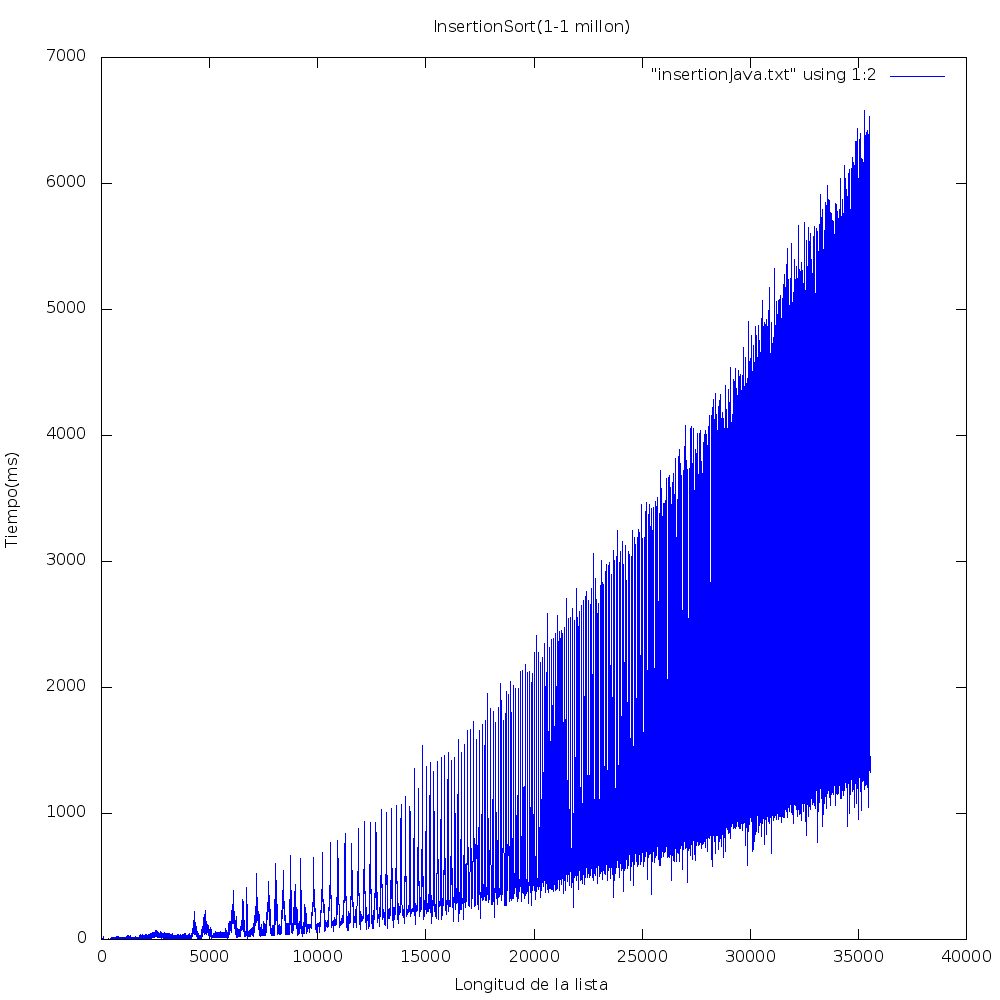
\includegraphics[trim=0cm 0cm 0cm 0cm, width=10cm]{1-1mIJava.png} 
          \caption{Gráfica para InsertionSort en el lenguaje Java de 1 a 1 millon}
      \end{figure}
      
       \begin{figure}[H]
         \centering
          %trim left bottom right top
          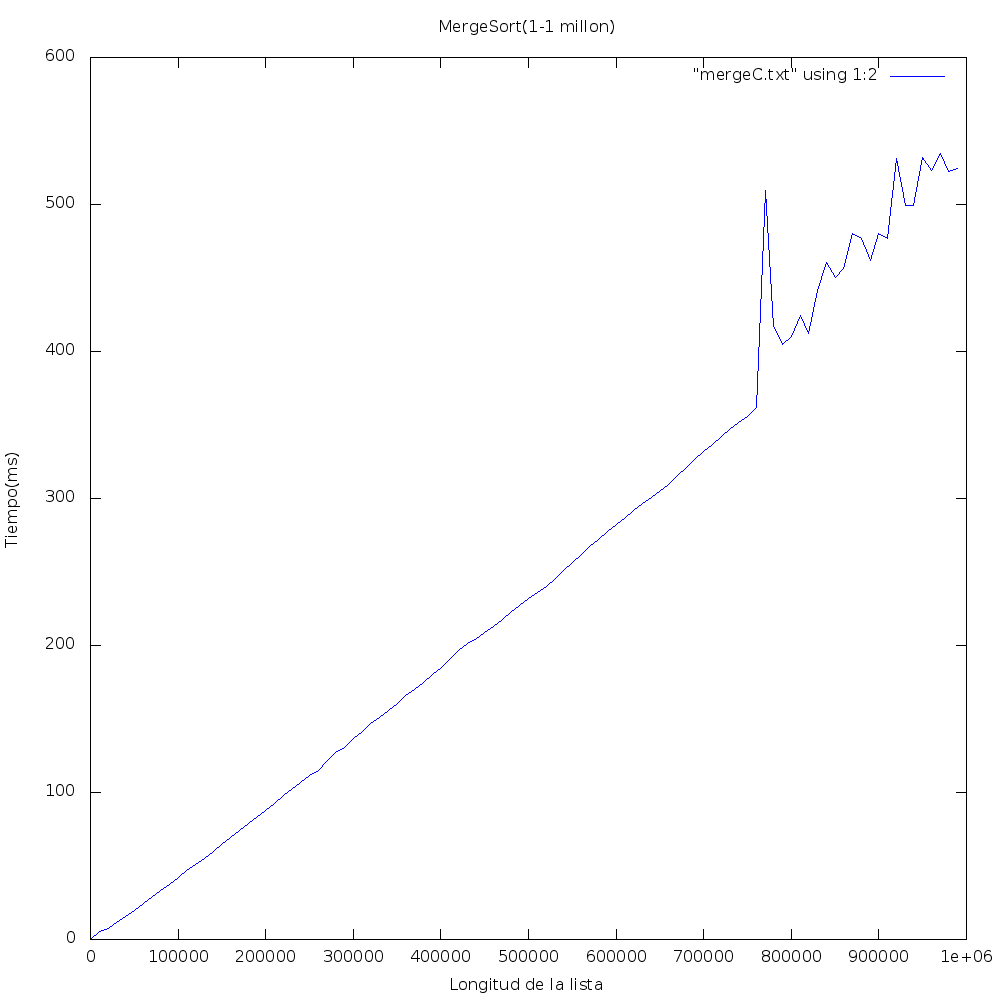
\includegraphics[trim=0cm 0cm 0cm 0cm, width=10cm]{1-1mC.png} 
          \caption{Gráfica para MergeSort en el lenguaje C de 1 a 1 millon}
      \end{figure}
       \begin{figure}[H]
         \centering
          %trim left bottom right top
          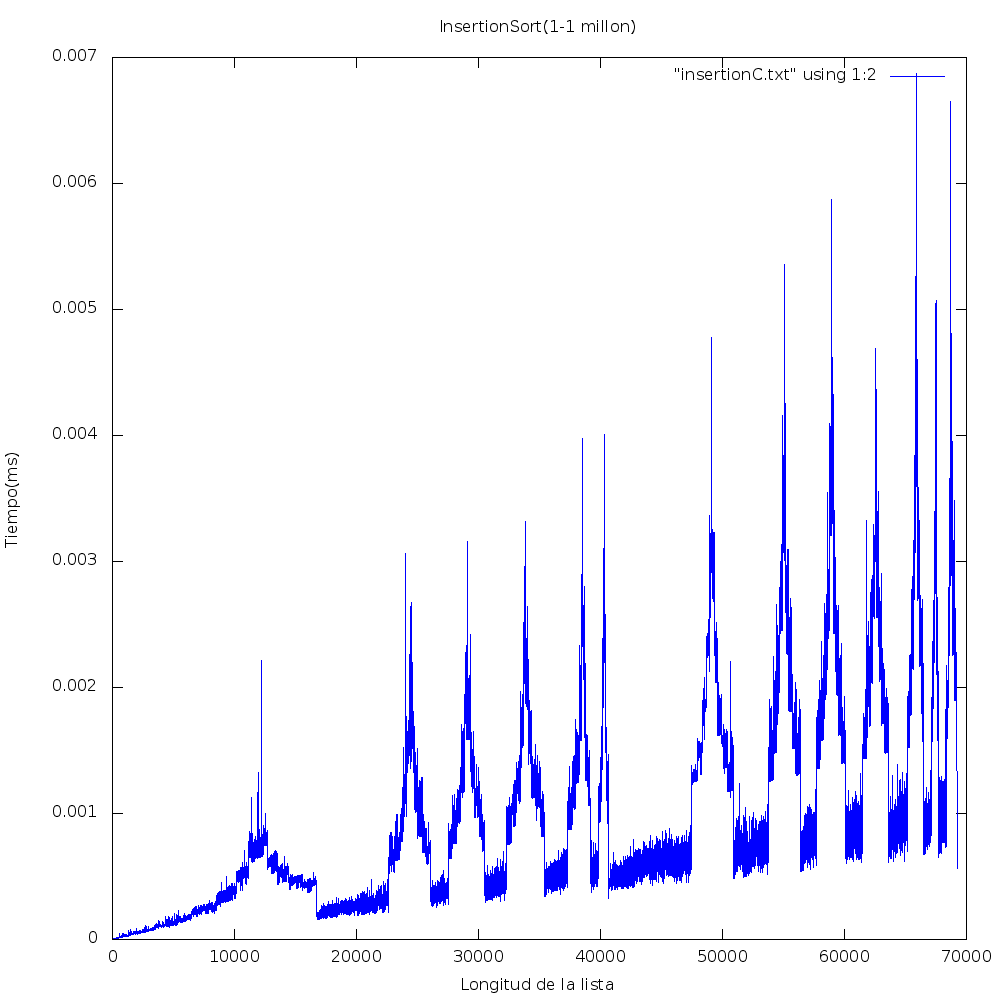
\includegraphics[trim=0cm 0cm 0cm 0cm, width=10cm]{1-1mIC.png} 
          \caption{Gráfica para InsertionSort en el lenguaje C de 1 a 1 millon}
      \end{figure}
       \begin{figure}[H]
         \centering
          %trim left bottom right top
          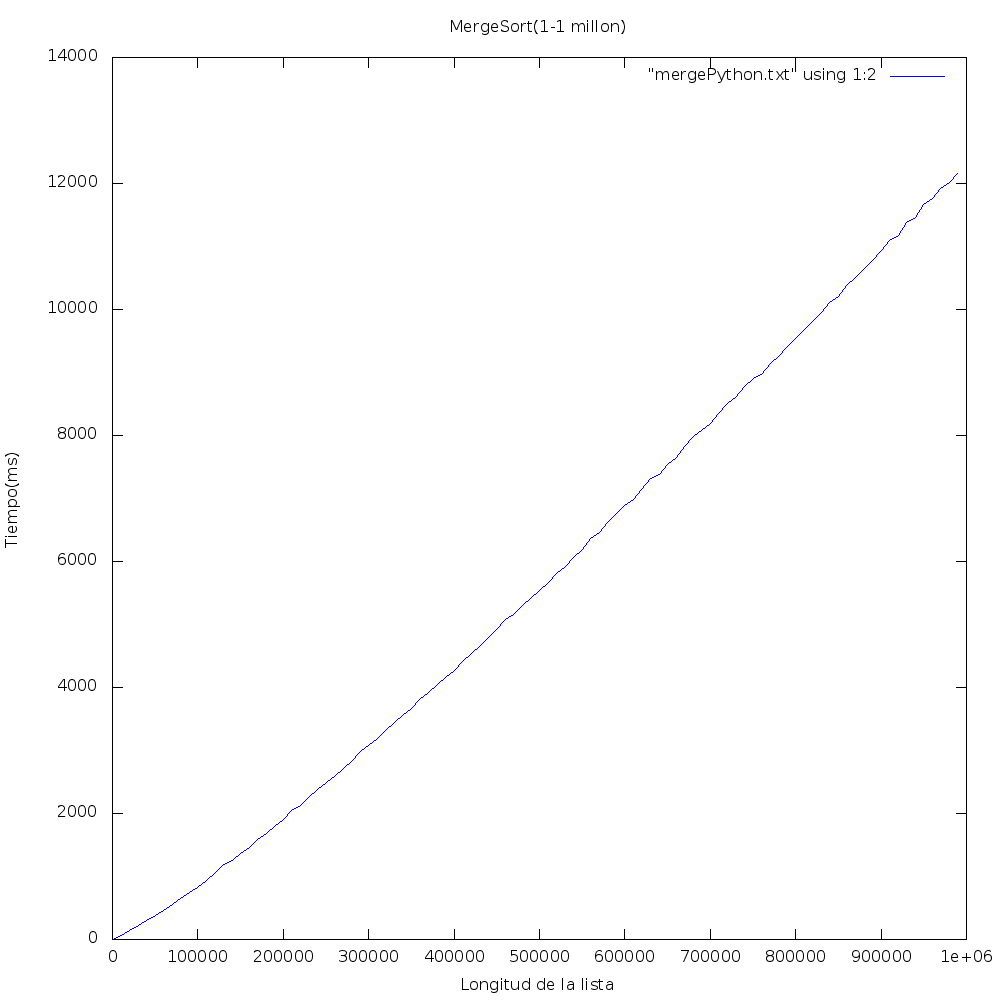
\includegraphics[trim=0cm 0cm 0cm 0cm, width=10cm]{1-1mPython.png} 
          \caption{Gráfica para MergeSort en el lenguaje Python de 1 a 1 millon}
      \end{figure}
       \begin{figure}[H]
         \centering
          %trim left bottom right top
          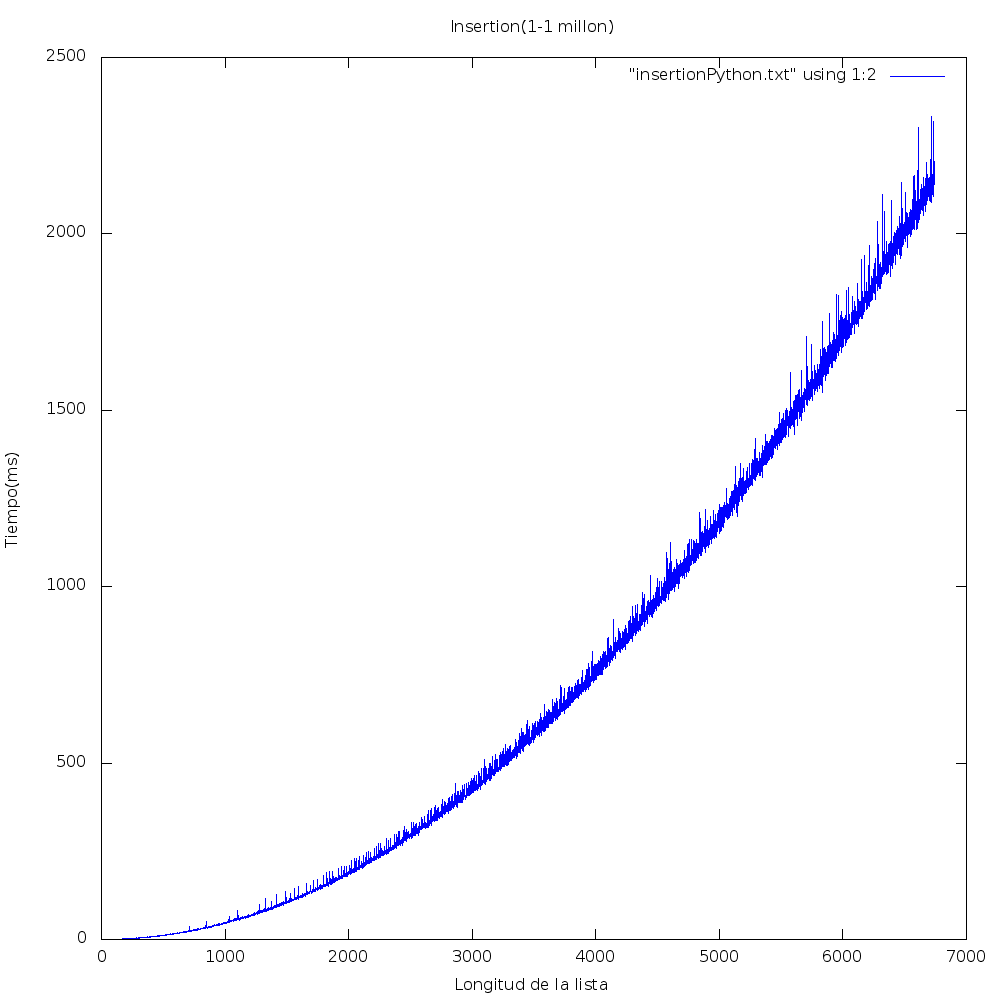
\includegraphics[trim=0cm 0cm 0cm 0cm, width=10cm]{1-1mIPython.png} 
          \caption{Gráfica para InsertionSort en el lenguaje Python de 1 a 1 millon}
      \end{figure}
      
  \begin{figure}[H]
         \centering
          %trim left bottom right top
          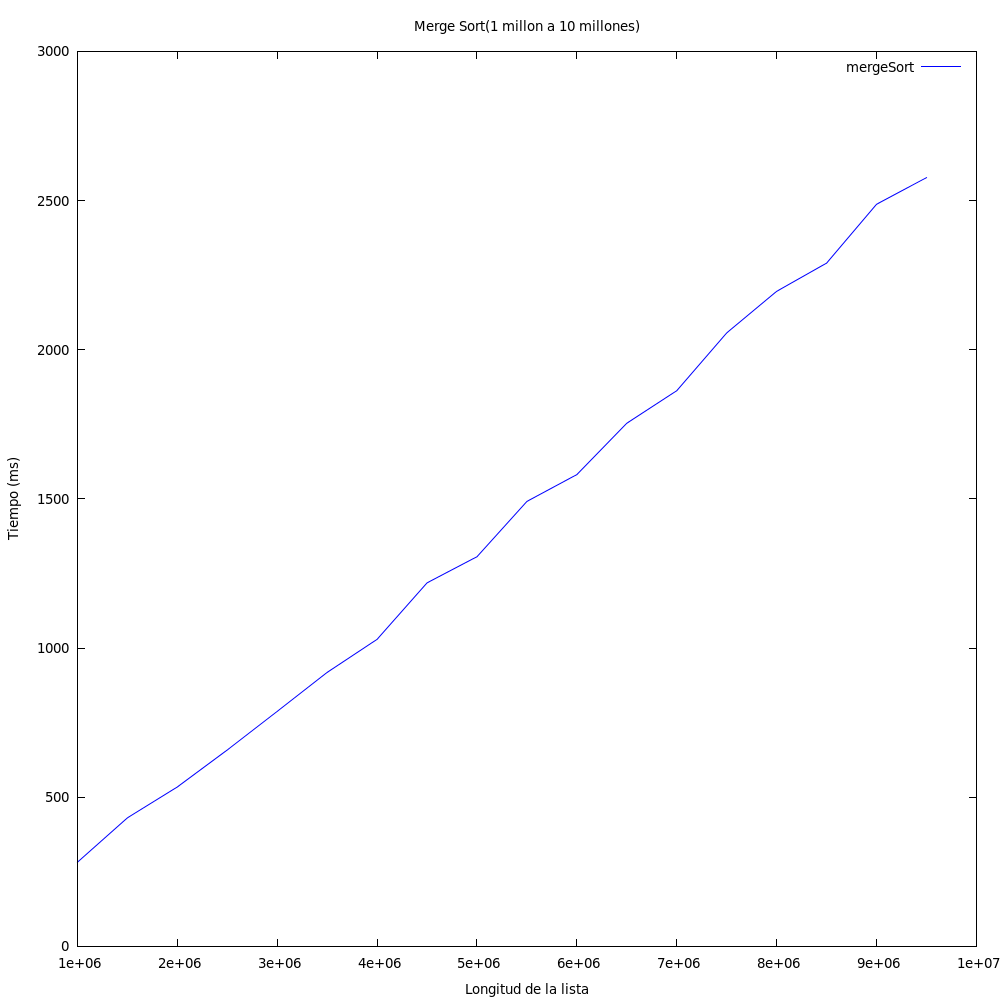
\includegraphics[trim=0cm 0cm 0cm 0cm, width=10cm]{1-10Java.png} 
          \caption{Gráfica para MergeSort en el lenguaje Java}
      \end{figure}
       \begin{figure}[H]
         \centering
          %trim left bottom right top
          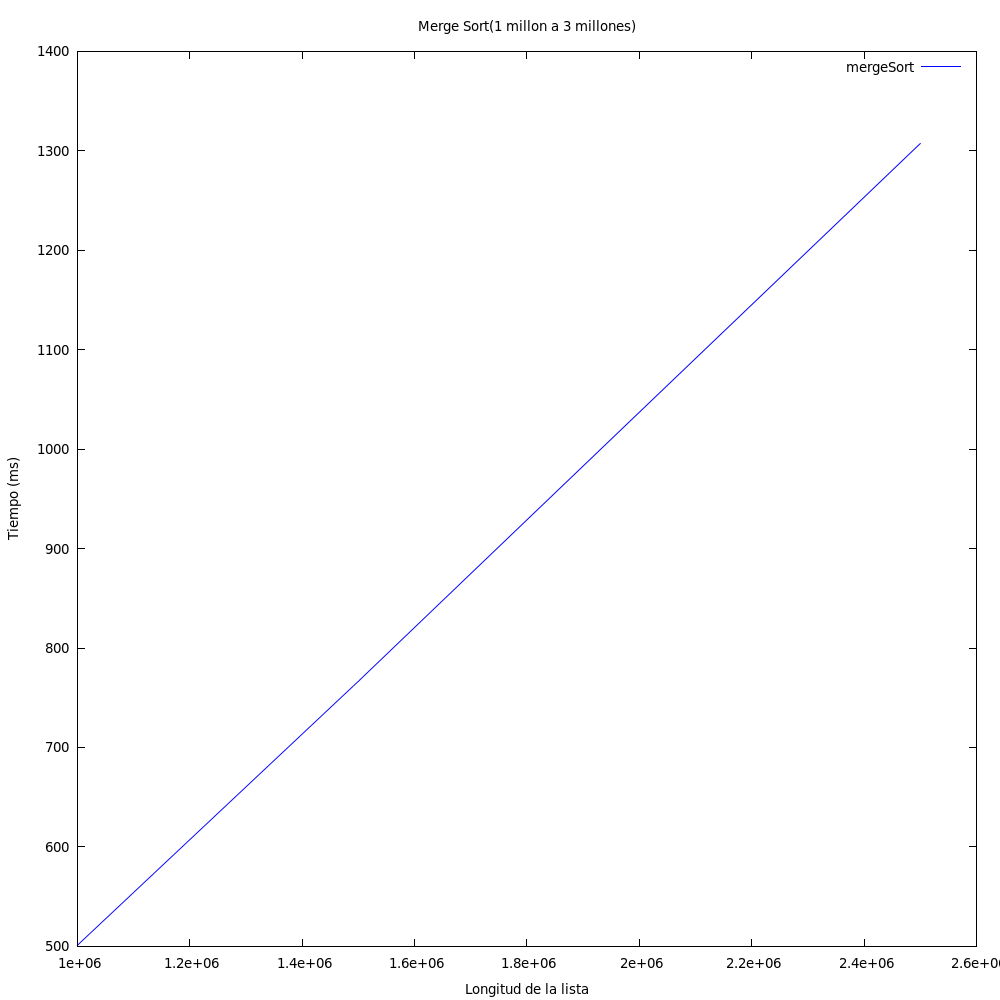
\includegraphics[trim=0cm 0cm 0cm 0cm, width=10cm]{1-2C.png} 
          \caption{Gráfica para MergeSort en el lenguaje C}
      \end{figure}
   \textbf{Nota:} No se agregó gráfica para InsertionSort ni para los programas en 
   python para cuando n vale más de un millón. Ya que, después de mucho tiempo ejecutandose
   o el sistema operativo mataba el thread o simplemente no acababa. 
   Máquina en la que se ejecuto el programa:
   \begin{itemize}
    \item  Equipo de escritorio
    \item Fabricante: Lenovo, de 64 bits
    \item CPU: Pentium(R) Dual-Core CPU E5400 @ 2.70GHz,
    \item fabricante del cpu: Intel Corp
    \item Capacidad: 2700MHz
    \item Reloj: 200MHz
    \item cache 0: capacidad 64KiB
    \item cache 1: capacidad 2MiB
    \item memoria Ram: tamaño 3GiB
   \end{itemize}

  



\end{enumerate}

\end{document}
